\documentclass[11pt]{article}

\usepackage[T1]{fontenc}
\usepackage{lmodern}
\usepackage[margin=1in]{geometry}
\usepackage{booktabs}
\usepackage{array}
\usepackage{longtable}
\usepackage{graphicx}
\usepackage{hyperref}
\usepackage{xurl}
\usepackage{xcolor}
\usepackage{tikz}
\usetikzlibrary{arrows.meta, positioning}
\usepackage{amsmath}
\usepackage{amssymb}
\usepackage{enumitem}
\usepackage{caption}
\usepackage{microtype}

\hypersetup{
    colorlinks=true,
    linkcolor=blue!50!black,
    urlcolor=blue!50!black,
    citecolor=blue!50!black
}
\urlstyle{tt}
\emergencystretch=2em

% Reusable column type for wrapped path/source cells in tables.
\newcolumntype{P}[1]{>{\raggedright\arraybackslash\ttfamily\scriptsize}p{#1}}

\title{\textbf{From a Bare Reach Template to Vision-Guided Pick-and-Place:\\
Reinforcement Learning for a Kinova Gen3 Manipulator in Isaac Lab}}
\author{Ido Raviel, Dan Butensky \\ \small Bar-Ilan University --- AI Excellence Program \\ \small Guided by Prof.\ Gal Kaminka}
\date{\today}

\begin{document}
\maketitle

\begin{abstract}
This report documents the development of a reinforcement-learning pick-and-place
pipeline for a Kinova Gen3 arm with a Robotiq 2F-140 gripper, built in NVIDIA Isaac
Lab and trained with PPO via \url{rsl_rl}. The project started from a generic,
gripper-less Isaac Lab reach template and progressed through: (1) hardware
integration of a parallel gripper, including an abandoned first attempt with a
2F-85 gripper before settling on the 2F-140; (2) an orientation-aware \emph{reach}
policy; (3) a \emph{grasp} policy that was first trained from a single canonical
start pose, found to fail when handed off from the reach policy in a chained
rollout, and then retrained with IK-randomized start states for robustness; (4) a
state-machine \emph{chain} that composes the two frozen policies into a full
reach~$\to$~grasp~$\to$~carry pick-and-place behavior; and (5) a vision-based
extension that trains a convolutional pose-estimation network (\url{CubePoseNet})
from a single fixed workspace camera and substitutes its live predictions for the
privileged, simulator-only cube pose used earlier in the pipeline. The report
presents the exact reward structures, PPO hyperparameters, and training curves for
each policy, explicitly separated from the simulated-environment (MDP) parameters
they are often confused with, every value traced to its defining file and, where the
two disagree, to the configuration actually saved with the shipped checkpoint;
several trial-and-error episodes that shaped the final design (a still-unresolved
reach-wavering artifact and the IK-seeding strategy that unlocked stable grasp
training); and the vision model's measured accuracy (0.50\,cm position error,
1.2\textdegree{} rotation error on a held-out test set, independently re-measured
while preparing this revision), together with an honest account of what has
\emph{not} yet been measured --- most notably, a persisted end-to-end success rate
for the chain.
\end{abstract}

\clearpage
\section*{Code Repository and Reproducibility}
\addcontentsline{toc}{section}{Code Repository and Reproducibility}
\label{sec:repo}

Every file path, parameter, and command in this report refers to a specific,
publicly available state of the project's code repository. This page exists so
that page is never in doubt.

\paragraph{Repository.} \url{https://github.com/IdoRaviel/kinova_isaaclab_sim2real}
(branch \url{main}). This repository extends
\href{https://github.com/louislelay/kinova_isaaclab_sim2real}{\url{louislelay/kinova_isaaclab_sim2real}},
an Isaac Lab reach-task template, with a full pick-and-place chain, a robustness-retrained
grasp policy, and the vision-based pose estimator described in
Section~\ref{sec:vision}.

\paragraph{Repository map.} The project is an Isaac Lab \emph{extension}
(a self-contained Python package Isaac Lab loads via entry points) plus a set of
standalone scripts that drive it.

\begin{center}
\renewcommand{\arraystretch}{1.25}
\begin{tabular}{P{4.6cm}P{9.4cm}}
\toprule
Path & Contents \\
\midrule
\url{source/gen3/} & The Isaac Lab extension package (installed with \url{pip install -e}). Its Python package root is \url{source/gen3/gen3/}. \\
\url{source/gen3/gen3/assets/} & Robot/gripper asset definition (\url{kinova_gen3_2f140.py}), the vendored USD and URDF files. \\
\url{source/gen3/gen3/tasks/manager_based/gen3_reach/} & The reach task: environment config, PPO config, and reach-specific MDP functions (rewards, events, curricula). \\
\url{source/gen3/gen3/tasks/manager_based/gen3_grasp/} & The grasp task: environment config, PPO config, reward/observation functions, and the IK-based reset. \\
\url{source/gen3/gen3/tasks/manager_based/gen3_lift_and_place/} & The single-policy lift-and-place task, the two-policy \emph{chain} environments (ground-truth and vision variants), and the camera + \url{CubePoseNet} inference code. \\
\url{scripts/rsl_rl/} & Train/play/eval entry points (\url{train.py}, \url{play.py}, \url{eval/eval.py}) and the chain runner (\url{play_lift_and_place.py}, configured by \url{lift_and_place_cfg.py}). \\
\url{scripts/rsl_rl/vision/} & The vision pipeline: dataset collection, splitting, training, and evaluation for \url{CubePoseNet} (pure PyTorch; no Isaac Sim needed except for collection). \\
\url{pretrained_models/} & Shipped checkpoints: \url{reach_with_orientation/}, \url{robust_grasp/} (each with \url{policy.pt}, \url{agent.yaml}, \url{env.yaml} --- the \emph{exact} configuration saved at training time, used throughout this report as the authoritative record of what produced each checkpoint), and \url{cube_pose/best.pt}. \\
\url{report/} & This report (\url{kinova_project_report.tex}). \\
\url{docs/} & Longer-form reference documentation (architecture, configuration, reproduction, vision pipeline) that this report draws on but does not duplicate. \\
\bottomrule
\end{tabular}
\end{center}

\paragraph{What is upstream vs.\ project code.} Three layers are in play throughout
this report, and tables below label every value with which layer it comes from:
(1) \textbf{NVIDIA Isaac Lab} (external framework, installed separately, not part of
this repository) supplies the simulation infrastructure, the manager-based
environment/config system, and the base \url{ReachEnvCfg} / \url{LiftEnvCfg}
classes this project subclasses; (2) \textbf{\url{rsl_rl}}
(\href{https://github.com/leggedrobotics/rsl_rl}{\url{leggedrobotics/rsl_rl}},
installed as the \url{rsl-rl-lib} package, version 5.0.1 in this project's
environment) supplies the PPO implementation itself; (3) \textbf{this repository}
supplies the robot/gripper integration, all three task configurations, every custom
reward/observation/reset function, the chain state machine, and the vision pipeline.
The project did not re-implement PPO, RSL-RL, or Isaac Lab's simulation core; the
project's contribution is everything layer (3) lists above, in particular the
IK-randomized grasp-reset design (Section~\ref{sec:grasp}) and the vision pipeline
(Section~\ref{sec:vision}).

\paragraph{Verified reproduction commands.} All commands are run from the repository
root with \url{conda activate env_isaaclab} active, after installing the
extension once via \url{python -m pip install -e source/gen3}.

\begin{center}
\renewcommand{\arraystretch}{1.15}
\begin{tabular}{P{5.4cm}P{8.6cm}}
\toprule
Command & What it does \\
\midrule
\url{python scripts/rsl_rl/play_lift_and_place.py} & Runs the full frozen reach$\to$grasp$\to$carry chain (Section~\ref{sec:chain}). Add \url{--vision} to drive it from \url{CubePoseNet} instead of ground truth. \\
\url{python scripts/rsl_rl/play.py --task Gen3-Reach-v0 --checkpoint pretrained_models/reach_with_orientation/policy.pt} & Runs the reach policy alone. \\
\url{python scripts/rsl_rl/play.py --task Gen3-Grasp-v0 --checkpoint pretrained_models/robust_grasp/policy.pt} & Runs the grasp policy alone. \\
\url{python scripts/rsl_rl/train.py --task Gen3-Reach-v0} & Retrains reach from scratch (Section~\ref{sec:reach}). \\
\url{python scripts/rsl_rl/train.py --task Gen3-Grasp-v0} & Retrains grasp from scratch (Section~\ref{sec:grasp}). \\
\url{python scripts/rsl_rl/vision/collect_vision_data.py --output_dir vision_dataset --num_frames 10000} & Collects the vision training dataset from chain rollouts (Section~\ref{sec:vision}). \\
\url{python scripts/rsl_rl/vision/split_vision_dataset.py --dataset_dir vision_dataset} & Splits the collected dataset into train/val/test. \\
\url{python scripts/rsl_rl/vision/train_cube_pose.py --dataset_dir vision_dataset} & Trains \url{CubePoseNet} (pure PyTorch, no Isaac Sim). \\
\url{python scripts/rsl_rl/vision/eval_cube_pose.py} & Evaluates a \url{CubePoseNet} checkpoint on the held-out test split; used to independently re-measure the accuracy numbers in Section~\ref{sec:vision}. \\
\bottomrule
\end{tabular}
\end{center}

\clearpage
\tableofcontents

% =====================================================================
\section{Introduction}
\label{sec:intro}
% =====================================================================

The goal of this project is to train a Kinova Gen3 robot arm, fitted with a Robotiq
2F-140 parallel gripper, to autonomously pick a cube up off a table and carry it to
a target pose in the air, using reinforcement learning trained entirely in
simulation (NVIDIA Isaac Lab). Rather than training a single monolithic policy for
the whole task, the
project decomposes it into two specialized policies --- \emph{reach} and
\emph{grasp} --- each trained independently with PPO, and then composes them at
inference time into a single behavior via an explicit state machine. A later phase
of the project replaces the privileged, simulator-only cube pose that both policies
initially rely on with a pose estimate produced by a learned vision model observing
a single fixed camera.

This report is organized to follow the project's actual chronology: Section~\ref{sec:reach}
covers the reach policy. Section~\ref{sec:grasp} covers the grasp policy, including its most
significant redesign. Section~\ref{sec:chain} covers the chain that combines both frozen
policies into pick-and-place. Section~\ref{sec:results} summarizes quantitative results across all
of the above. Section~\ref{sec:vision} covers the vision-based pose estimation work. Section~\ref{sec:further}
covers further development (handling the reach-wavering artifact and
sim-to-real deployment). Section~\ref{sec:conclusion} is a brief conclusion. See the
``Code Repository and Reproducibility'' page immediately before this table of
contents for the repository and a map of where each part of the system lives in
the codebase.

\subsection{Background: PPO, RSL-RL, and Isaac Lab}
\label{sec:background}

\paragraph{Reinforcement learning setup.} Each task in this project (reach, grasp)
is formulated as a Markov Decision Process (MDP): at every control step the agent
observes a state (joint positions/velocities, commanded target, and task-specific
quantities such as the cube's pose), chooses a continuous action (target joint
positions, plus a binary gripper command for grasp), and receives a scalar reward
computed from the resulting simulated physics state. The MDP's observation space,
action space, reward function, reset distribution, and episode horizon are all
defined by the \emph{environment configuration} for that task (Sections~\ref{sec:reach}
and~\ref{sec:grasp} give the exact values and their source files) --- this is
distinct from the \emph{learning algorithm} used to train a policy for that MDP,
described next. Because the policy conditions only on its own observation vector,
not the simulator's full internal state, the setting is more precisely a partially
observed MDP; the project does not rely on this distinction beyond noting it here.

\paragraph{PPO.} Every policy in this project is trained with Proximal Policy
Optimization (PPO) (Schulman et al., 2017), an on-policy actor-critic algorithm. At
a high level: an \emph{actor} network maps observations to a distribution over
actions (here, a diagonal Gaussian over continuous joint-position targets), and a
separate \emph{critic} network estimates the state-value function used to reduce
the variance of the policy gradient. Training alternates between (1) collecting a
batch of \emph{rollouts} --- fixed-length trajectories from many parallel simulated
environments, run under the current policy --- and (2) computing an
\emph{advantage} estimate for each visited state-action pair via Generalized
Advantage Estimation (GAE), then (3) taking several gradient-ascent epochs over
that batch on PPO's \emph{clipped surrogate objective}
\[
L^{\text{CLIP}}(\theta) = \mathbb{E}_t\!\left[\min\!\big(r_t(\theta)\,\hat{A}_t,\;
\operatorname{clip}(r_t(\theta),\,1-\epsilon,\,1+\epsilon)\,\hat{A}_t\big)\right],
\]
where $r_t(\theta) = \pi_\theta(a_t\mid s_t) / \pi_{\theta_{\text{old}}}(a_t\mid s_t)$
is the probability ratio between the updated and the rollout-time policy, $\hat A_t$
is the GAE advantage estimate, and $\epsilon$ is the clip parameter (0.2 throughout
this project; see the PPO tables in Sections~\ref{sec:reach} and~\ref{sec:grasp}).
Clipping the objective when $r_t$ moves too far from 1 caps how much a single update
can change the policy at a state where the new-vs-old probability ratio has already
moved a lot, which is what makes PPO robust to the large batches and many epochs per
batch used here without a separate trust-region constraint.

\paragraph{RSL-RL.} PPO itself is not implemented by this project. Training uses
\href{https://github.com/leggedrobotics/rsl_rl}{RSL-RL}
(package \url{rsl-rl-lib}, version 5.0.1), an open-source PPO implementation from
ETH Zurich's Robotic Systems Lab, integrated into Isaac Lab via the
\url{isaaclab_rl.rsl_rl} wrapper. Every ``PPO hyperparameters'' table in this
report (Sections~\ref{sec:reach} and~\ref{sec:grasp}) is a project-authored
configuration of RSL-RL's \url{RslRlPpoAlgorithmCfg}, \url{RslRlPpoActorCriticCfg},
and \url{RslRlOnPolicyRunnerCfg} classes, one \url{*_ppo_cfg.py} file per
task; the algorithm code they configure is RSL-RL's, not this project's.

\paragraph{Isaac Lab.} The simulation environment, physics stepping, GPU-parallel
scene cloning, and the manager-based configuration system (observation/action/reward/
termination/event/curriculum managers, all configured via Python dataclasses) are
supplied by NVIDIA Isaac Lab (Mittal et al., 2025), version 2.3.2 in this
project's environment. This project's three tasks are Isaac Lab
\url{ManagerBasedRLEnv} subclasses; Sections~\ref{sec:reach} and~\ref{sec:grasp}
distinguish, for every parameter, whether it is set by this project's task
configuration or inherited unchanged from an Isaac Lab base class.

% =====================================================================
\section{Reach Policy}
\label{sec:reach}
% =====================================================================

\subsection{Task and algorithm}

The reach policy commands the arm's seven joints so that the gripper's fingertip
frame (the \url{ee_frame}, offset 0.21\,m from the wrist flange --- not the
flange itself; this offset is the constant \url{FINGERTIP_OFFSET_M} in
\url{source/gen3/gen3/assets/kinova_gen3_2f140.py}, shared by all three tasks)
tracks a randomly sampled target position \emph{and orientation}.
Orientation tracking was added specifically so the policy could learn to approach
the cube top-down, which the grasp policy requires for a reliable handoff.

The reach task is defined by two files, which this report keeps separate throughout
because they configure two different things:
\begin{itemize}
    \item \url{source/gen3/gen3/tasks/manager_based/gen3_reach/joint_pos_env_cfg.py}
    defines \url{Gen3ReachEnvCfg}, the class \emph{the MDP itself} --- observations,
    actions, rewards, resets, episode horizon, and the number/layout of parallel
    simulated environments. It subclasses Isaac Lab's \url{ReachEnvCfg}
    (installed with Isaac Lab, at
    \url{isaaclab_tasks/manager_based/manipulation/reach/reach_env_cfg.py} in an
    Isaac Lab checkout; not part of this repository) and overrides the parts specific
    to the Gen3 + 2F-140 hardware and the fingertip-tracking convention, while several
    values --- notably the parallel-environment count, environment spacing, and
    episode length --- are left at the parent class's values (Table~\ref{tab:reach_mdp}
    marks each explicitly).
    \item \url{source/gen3/gen3/tasks/manager_based/gen3_reach/agents/rsl_rl_ppo_cfg.py}
    defines \url{Gen3ReachPPORunnerCfg}, the \emph{learning-algorithm} configuration
    consumed by RSL-RL's on-policy runner (Section~\ref{sec:background}) --- network
    sizes, PPO's own coefficients, and the training budget. It has no effect on what
    the MDP is; it only affects how a policy is fit to it.
\end{itemize}

Table~\ref{tab:reach_mdp} lists the simulation/MDP-level parameters and
Table~\ref{tab:reach_ppo} lists the PPO/algorithm-level parameters, each with an
explicit source. Both are cross-checked against
\url{pretrained_models/reach_with_orientation/env.yaml} and \url{agent.yaml}
--- the full environment and runner configuration Isaac Lab serializes at the start
of training, saved alongside the shipped \url{policy.pt} --- which is the
authoritative record of what configuration actually produced that checkpoint,
since the checkpoint could in principle have been trained under an older version of
the source files than the ones currently in the repository.

\begin{table}[h]
\centering
\caption{Reach task: simulation and MDP parameters (\emph{not} PPO hyperparameters --- see
Table~\ref{tab:reach_ppo} for those). ``Inherited'' means the value comes from Isaac
Lab's \url{ReachEnvCfg} unchanged; \url{Gen3ReachEnvCfg} does not override it.}
\label{tab:reach_mdp}
\begin{tabular}{P{3.1cm}P{2.1cm}P{2.5cm}P{5.6cm}}
\toprule
Parameter & Code default & Checkpoint's \url{env.yaml} & Source \\
\midrule
Parallel environments & 4096 (inherited) & \textbf{2048} & \url{ReachEnvCfg.scene} (Isaac Lab); overridden at train time via \url{--num_envs} \\
Environment spacing & 2.5\,m (inherited) & 2.5\,m & \url{ReachEnvCfg.scene} (Isaac Lab) \\
Episode length & 12.0\,s (inherited) & 12.0\,s & \url{ReachEnvCfg.__post_init__} (Isaac Lab) \\
Control decimation & 2 (inherited) & 2 & \url{ReachEnvCfg.__post_init__} (Isaac Lab) \\
Physics step \url{sim.dt} & 1/60\,s (inherited) & 1/60\,s & \url{ReachEnvCfg.__post_init__} (Isaac Lab) \\
\bottomrule
\end{tabular}
\end{table}

\textbf{On the 4096-vs-2048 discrepancy.} The number of parallel environments is
\emph{not} set anywhere in this project's reach files: \url{Gen3ReachEnvCfg} never
touches \url{self.scene.num_envs}, so its effective value is whatever Isaac
Lab's own \url{ReachEnvCfg} sets, which is 4096. That is the value a fresh
\url{python scripts/rsl_rl/train.py --task Gen3-Reach-v0} run would use today.
However, the \url{env.yaml} actually saved with the shipped
\url{reach_with_orientation} checkpoint records \url{num_envs: 2048} ---
meaning that specific training run was launched with an explicit
\url{--num_envs 2048} override (\url{scripts/rsl_rl/train.py} applies any
\url{--num_envs} CLI value on top of the config default), most plausibly to fit
within a smaller GPU's memory. Both numbers are real and verified, but they answer
different questions: 4096 is what the checkpointed \emph{code} defaults to today,
2048 is what actually produced the shipped \emph{policy}. Environment spacing
(2.5\,m) is the physical distance Isaac Lab places between cloned parallel scene
instances in the simulator so they do not overlap or physically interact --- it has
no relationship to PPO's optimization equations and is unaffected by the
environment-count override.

\begin{table}[h]
\centering
\caption{Reach policy: PPO / policy-architecture / training-runner parameters, from
\url{gen3_reach/agents/rsl_rl_ppo_cfg.py} (full path:
\url{source/gen3/gen3/tasks/manager_based/gen3_reach/agents/rsl_rl_ppo_cfg.py}),
class \url{Gen3ReachPPORunnerCfg}. Identical to the saved \url{agent.yaml}.}
\label{tab:reach_ppo}
\begin{tabular}{lll}
\toprule
Parameter & Value & Category \\
\midrule
Actor/critic network & MLP $[64, 64]$, ELU activation & policy architecture \\
Initial action noise std & 1.0 & policy architecture \\
Steps per environment per update & 24 & runner \\
Learning epochs per update & 8 & PPO \\
Mini-batches per update & 4 & PPO \\
Learning rate & $1\times10^{-3}$, adaptive (target KL 0.01) & PPO \\
Discount factor $\gamma$ & 0.99 & PPO \\
GAE $\lambda$ & 0.95 & PPO \\
PPO clip parameter $\epsilon$ & 0.2 & PPO \\
Entropy coefficient & 0.001 & PPO \\
Value loss coefficient & 1.0 (clipped value loss) & PPO \\
Max gradient norm & 1.0 & PPO \\
Empirical obs./action normalization & disabled & runner \\
Max training iterations & 1500 & runner \\
\bottomrule
\end{tabular}
\end{table}

\subsection{Reward structure}

Table~\ref{tab:reach_rewards} lists every reward term. Position and orientation tracking each
use a coarse L2 term (always penalizing error) plus a fine-grained tanh-shaped bonus
term (rewarding precise alignment near the target), a standard Isaac Lab pattern; the
coarse/fine pair for the \emph{fingertip} (rather than Isaac Lab's stock wrist-flange
version) is implemented by this project in
\url{source/gen3/gen3/tasks/manager_based/gen3_reach/mdp/rewards.py}
(functions \url{ee_position_command_error}, \url{ee_position_command_error_tanh},
\url{ee_orientation_command_error}, \url{ee_orientation_command_error_tanh}) and
wired to the environment, with its weight, in
\url{gen3_reach/joint_pos_env_cfg.py}. Concretely, the fine-grained position term
computes $1-\tanh(\lVert p_{\text{fingertip}} - p_{\text{target}}\rVert / \text{std})$
(std $=0.07$\,m) and the coarse term is the unshaped L2 norm; the orientation terms are
the analogous shortest-path-angle versions.
Two smoothness terms are introduced via a \emph{curriculum} --- implemented by this
project's \url{modify_reward_weight_ramp} function in
\url{gen3_reach/mdp/curriculums.py} (Isaac Lab supplies only a step-change
curriculum, \url{modify_reward_weight}; the linear ramp is project code) --- that ramps
their weight linearly from 0 at 25\% of training to their final value at 60\% of
training, so that early exploration is not suppressed by a smoothness penalty before
the policy has learned to reach at all. To change any reward weight, edit its
\url{RewTerm(..., weight=...)} call in \url{joint_pos_env_cfg.py}; to change
what a term computes, edit the corresponding function in \url{mdp/rewards.py}.

\begin{table}[h]
\centering
\caption{Reach policy: reward terms and weights. ``Wired in'' is where the weight is
set; ``Implemented in'' is where the function's math lives. Both paths are relative to
\url{source/gen3/gen3/tasks/manager_based/gen3_reach/}.}
\label{tab:reach_rewards}
\begin{tabular}{P{4.6cm}P{2.3cm}P{2.6cm}P{2.6cm}}
\toprule
Term & Weight & Wired in & Implemented in \\
\midrule
\url{end_effector_position_tracking} & $-0.6$ & \url{joint_pos_env_cfg.py} & \url{mdp/rewards.py} \\
\url{end_effector_position_tracking_fine_grained} & $+0.6$ (std 0.07\,m) & \url{joint_pos_env_cfg.py} & \url{mdp/rewards.py} \\
\url{end_effector_orientation_tracking} & $-0.3$ & \url{joint_pos_env_cfg.py} & \url{mdp/rewards.py} \\
\url{end_effector_orientation_tracking_fine_grained} & $+0.30$ (std 0.5\,rad) & \url{joint_pos_env_cfg.py} & \url{mdp/rewards.py} \\
\url{action_rate} & $0 \to -0.005$ (curriculum) & \url{joint_pos_env_cfg.py} & Isaac Lab (\url{mdp.action_rate_l2}) \\
\url{joint_vel} & $0 \to -0.0015$ (curriculum) & \url{joint_pos_env_cfg.py} & Isaac Lab (\url{mdp.joint_vel_l2}) \\
\bottomrule
\end{tabular}
\end{table}

\subsection{Randomization}

To make the reach policy robust to the states the grasp policy and the eventual
chain would present it with, several quantities are randomized every episode via
\url{EventTermCfg} entries in \url{gen3_reach/joint_pos_env_cfg.py} (an MDP
reset-event configuration, not a PPO setting):

\begin{itemize}
    \item \textbf{Gripper state:} randomized open/closed at every reset via this
    project's \url{reset_joints_held_uniform} (\url{gen3_reach/mdp/events.py}
    --- unlike Isaac Lab's stock \url{reset_joints_by_offset}, it also writes the
    PD drive target, so the stiff finger joint actually holds the sampled position
    instead of snapping back), so the
    policy learns to reach correctly whether or not it is already holding an
    object.
    \item \textbf{Payload mass:} an extra $0$--$0.3$\,kg is added to the gripper
    base link at random (the cube itself weighs 0.216\,kg, comfortably inside this
    range), and the policy does not observe the mass directly --- it must be
    robust to the load rather than compensate for a known value.
    \item \textbf{Target orientation range:} roll $\pm10^\circ$; pitch
    $120^\circ$--$180^\circ$ (with $180^\circ$, i.e.\ straight down, always
    included, since a top-down approach is required for grasping); yaw
    $\pm45^\circ$ (covers all four faces of the cube).
    \item \textbf{Target position range:} height $z \in [0.05, 0.50]$\,m.
\end{itemize}

% =====================================================================
\section{Grasp Policy}
\label{sec:grasp}
% =====================================================================

The grasp policy takes over once the arm is positioned above the cube (as handed
off by the reach policy, or by the chain's state machine) and is responsible for
lowering onto the cube, closing the gripper, and lifting it clear of the table.
Unlike reach, grasp went through a substantial redesign driven directly by a
failure discovered when the two policies were first chained together. As with
reach, the task's MDP is defined in
\url{source/gen3/gen3/tasks/manager_based/gen3_grasp/joint_pos_env_cfg.py}
(class \url{Gen3GraspEnvCfg}, subclassing Isaac Lab's \url{LiftEnvCfg}), and
its PPO/runner configuration separately in
\url{gen3_grasp/agents/rsl_rl_ppo_cfg.py} (class \url{Gen3GraspPPORunnerCfg}).
\url{LiftEnvCfg} sets \url{scene.num_envs=4096}, \url{env_spacing=2.5\,m}
and (in its own \url{__post_init__}) \url{episode_length_s=5.0}; none of
these three are overridden locally, so --- as with reach --- they are inherited, and
the checkpoint's saved \url{env.yaml} again shows \url{num_envs: 2048} (the
same GPU-driven override) with \url{env_spacing} and \url{episode_length_s}
unchanged from the inherited values. \url{Gen3GraspEnvCfg} does override the
physics step to \url{sim.dt=1/60\,s} (\url{LiftEnvCfg}'s own default is
0.01\,s/100\,Hz), so that the grasp environment runs at the same control frequency
as reach and the chain.

\subsection{Version (a): canonical-start baseline}
\label{sec:grasp_a}

The first working version of grasp was trained from a single, near-fixed starting
condition: the cube spawned at a fixed table position, $[0.43, 0, 0.055]$, with
only a small $\pm1$\,cm reset jitter in $x$ and $y$ (none in $z$), and the arm
always started from the same canonical joint configuration directly above it. Its
reward structure is summarized in Table~\ref{tab:grasp_rewards} (column ``Pre-retrain''),
and it trained successfully in isolation: given exactly the start condition it was
trained on, the policy reliably grasped and lifted the cube.

\textbf{The problem:} in a chained rollout, the reach policy does not hand off from
one single canonical joint configuration --- it arrives above the cube from a wide
variety of valid arm configurations (whatever the orientation- and
payload-randomized reach policy happens to produce). Grasp version~(a), having
only ever seen one starting condition, was not robust to this variation and failed
when actually chained after reach.

\subsection{Version (b): IK-randomized start states}

The fix was to retrain grasp so that every episode resets to a random, physically
valid start state: a random cube pose on the table, with the arm's joints IK-placed
so the gripper sits directly top-down above the cube. This is implemented in
\url{source/gen3/gen3/tasks/manager_based/gen3_grasp/mdp/ik_reset.py}
(function \url{reset_above_cube_ik}, wired into the environment as an
\url{EventTermCfg} in \url{joint_pos_env_cfg.py}). This is one of the
project's central contributions --- it is not part of Isaac Lab or the upstream
template.

\subsubsection{IK mechanism}

Inverse kinematics (IK) answers a simple question: given a desired position and
orientation for the gripper, what joint angles make the arm reach it? \url{ik_reset.py}
implements a hand-written, batched, damped-least-squares IK solver over a
\url{pytorch_kinematics} forward-kinematics/Jacobian chain built from a vendored
URDF (\url{source/gen3/gen3/assets/urdf/gen3_2f85.urdf}, FK-verified to match the
2F-140 USD's arm kinematics --- the gripper model itself is irrelevant to arm IK).
At startup it precomputes, for many randomly sampled cube poses on the table, a
matching valid arm configuration with the gripper placed directly top-down above
the cube, building a large bank of realistic, varied starting states for training
the grasp policy instead of relying on a single hand-picked canonical start pose.

Two refinements to this basic idea mattered in practice, both in the \url{solve}
method of the \url{_ArmIK} class in \url{ik_reset.py}:

\begin{itemize}
    \item A \textbf{decaying null-space pull toward the canonical pose} is added
    during the solve: $k_{\text{null}} = 0.6 \times (1 - \text{iter}/120)$, i.e.\ it
    starts at 0.6 and decays linearly to 0 across the 120 iterations. This keeps
    the (kinematically redundant) arm's null-space motion biased toward a natural,
    canonical-like configuration early in the solve, while still letting the
    position/orientation task term converge tightly by the end.
    \item Seeds themselves are initialized near the canonical joint configuration
    $[0, 0.3, 0, 1.8, 0, 0.7, 0]$ (this is not a separate hardcoded constant but is
    read directly from the robot asset's own default pose,
    \url{KINOVA_GEN3_2F140_CFG.init_state.joint_pos}, so it cannot silently
    drift out of sync with the arm's actual spawn pose) plus uniform noise
    (0.5\,rad), rather than fully random --- and among the seeds that converge, the
    solver picks the one with \textbf{minimum L2 distance to the canonical
    configuration}. The environment config calls \url{reset_above_cube_ik}
    with \url{num_seeds=8} (the function's own default of 4 is overridden).
    \item To keep training fast, IK is not solved live at every reset. It is run
    once at startup to build a table of 10{,}000 precomputed valid start
    states (built in chunks of 2500 to bound GPU memory, cached per device), and
    each subsequent episode reset simply samples a row from this table --- these
    two figures (\url{n_samples=10000}, \url{chunk=2500}) are the literal
    default arguments of \url{_build_start_table} in \url{ik_reset.py}.
\end{itemize}

\paragraph{Why the null-space pull and closest-to-canonical selection mattered.}
An early version of the IK reset, without this seeding and selection strategy,
produced \textbf{contorted} start poses --- valid IK solutions, but kinematically
unnatural ones. Training from these caused the arm to perform a visible
``circle/unwind'' motion at the start of every episode as it worked its way out of
the contorted configuration, and learning stalled under this regime. Seeding IK
near canonical, decaying the null-space pull rather than holding it fixed, and
explicitly selecting the seed closest to canonical among converged solutions
together produced natural, elbow-up start poses and was the single change that
most improved training progress --- learning proceeded noticeably faster than
under the contorted-pose regime. This specific comparison (contorted-pose regime
vs.\ the current seeding strategy) predates the two retrain versions described in
Table~\ref{tab:grasp_rewards} and is not preserved as a separate, buildable
version in the repository; it is reported here as a design account from the
project's working notes, not as a re-runnable experiment.

\paragraph{Training-speed note.} Solving IK live at every reset was reported at the
time to run at roughly 7 seconds per training iteration, which is far too slow for
RL training; switching to the precomputed table restored training throughput to
approximately 58{,}000 environment steps per second (full simulation speed). These
two throughput figures are carried over from earlier project notes rather than
independently re-benchmarked while preparing this report, and should be read as
recalled order-of-magnitude figures rather than freshly measured ones.

An additional \textbf{cube jitter} of $\pm4$\,cm (the \url{cube_jitter} parameter
of \url{reset_above_cube_ik}, added in version 2 of the retrain, see below) was
applied laterally to the cube's placement on top of the randomized start state,
specifically so the policy has to localize the cube rather than assume it sits
directly beneath the gripper.

\subsubsection{Reward retuning}
\label{sec:grasp_reward_retune}

Table~\ref{tab:grasp_rewards} traces every reward-weight change across the
robustness retrain to which of two successive versions of the grasp task
introduced it, rather than presenting an unsourced ``before/after.'' The retrain
happened in two steps: \emph{version 1} introduced the IK-based reset and a first
reward retune, and \emph{version 2} finalized it with cube jitter and a second
round of tuning; \emph{version 2 is the version currently on \url{main}}. The
``Version 2 (current)'' column matches both the current source and the
\url{robust_grasp} checkpoint's saved
\url{env.yaml} exactly. To modify a weight, edit the corresponding
\url{RewTerm(..., weight=...)} in \url{gen3_grasp/joint_pos_env_cfg.py};
to modify what a term computes, edit the function in
\url{gen3_grasp/mdp/rewards.py} (three of the four distance terms below are
implemented there; \url{lifting_object} calls Isaac Lab's own
\url{object_is_lifted}).

\begin{table}[h]
\centering
\caption{Grasp policy: reward weights across the robustness retrain, sourced to
which of the two retrain versions made each change. All functions are in
\url{gen3_grasp/mdp/rewards.py} unless marked (Isaac Lab).}
\label{tab:grasp_rewards}
\begin{tabular}{P{4.6cm}P{2.9cm}P{2.9cm}P{2.9cm}}
\toprule
Term & Pre-retrain & Version 1 & Version 2 (current) \\
\midrule
\url{lifting_object} (Isaac Lab \url{object_is_lifted}) & disabled & $+1.0$, h.\ 0.08\,m & $+1.0$, h.\ 0.05\,m \\
\url{ee_to_cube_l2} (coarse) & --- (did not exist) & $-1.0$ (new) & $-1.0$ \\
\url{ee_to_cube} (tanh, std 0.1) & $-0.2$ & $-0.2$ (unchanged) & $-0.2$ \\
\url{cube_to_target} (L2) & $-1.0$ & $-2.0$ & $-1.0$ \\
\url{cube_to_target_fine} (tanh, std 0.1) & $+0.25$ & $+0.50$ & $+1.0$ \\
\url{action_rate} curriculum target & $-5\times10^{-4}$ & $-5\times10^{-4}$ (unchanged) & $-1\times10^{-3}$ \\
\url{joint_vel} curriculum target & (not separately tuned) & $-5\times10^{-4}$ & $-5\times10^{-4}$ (unchanged) \\
Max training iterations (\url{agents/rsl_rl_ppo_cfg.py}) & 1000 & 1000 (unchanged) & 1300 \\
\bottomrule
\end{tabular}
\end{table}

Mathematically, the four custom terms above (from \url{mdp/rewards.py}) are:
\url{ee_to_cube_l2}$\;=\; \lVert p_{\text{ee}}-p_{\text{cube}}\rVert$ (raw L2, a
constant, non-saturating gradient toward the cube at any range);
\url{ee_to_cube}$\;=\;\tanh(\lVert p_{\text{ee}}-p_{\text{cube}}\rVert / 0.1)$
(near 0 close up, near 1 far away --- used with a \emph{negative} weight, so it is a
penalty that vanishes as the fingertip reaches the cube);
\url{cube_to_target}$\;=\;\lVert p_{\text{cube}}-p_{\text{target}}\rVert$ (raw L2
toward the commanded place target); and
\url{cube_to_target_fine}$\;=\;1-\tanh(\lVert p_{\text{cube}}-p_{\text{target}}\rVert / 0.1)$
(a positive bonus, used with a \emph{positive} weight, that is near zero past
$\sim$20\,cm and rises steeply inside $\sim$10\,cm). The coarse+fine pairing gives a
constant gradient far from the goal (so the agent is never in a flat reward region)
and a sharp signal up close (so it learns precision) --- the same pattern used for
reach in Section~\ref{sec:reach}.

The most significant single change is \textbf{re-enabling \url{lifting_object}}
(a hard, non-shaped $+1$ reward for every step the cube's height exceeds a small
threshold; the underlying function, \url{object_is_lifted}, is Isaac Lab's own,
re-exported via \url{gen3_grasp/mdp/__init__.py}'s
\url{from isaaclab_tasks...lift.mdp import *}), which was disabled in version~(a)
and had previously been removed altogether in an even earlier iteration of the
grasp task's reward design (a term then named \url{object_lifted_binary}).
Re-adding it was
specifically motivated by a \textbf{local optimum} the policy fell into without it:
hovering or orbiting near the cube, collecting the shaped distance rewards, without
ever actually committing to grasp and lift. Alongside it, version 1 added the
new coarse L2 term \url{ee_to_cube_l2} to strengthen the pull toward the cube
before the fine tanh term takes over at close range, and version 2 shrunk the
place-target height range from a tall $[0.30, 0.65]$\,m column down to a much
shallower $[0.08, 0.20]$\,m band (an MDP command-range change in
\url{joint_pos_env_cfg.py}, not a reward weight), making the ``carry it
somewhere reasonable'' part of the task substantially easier so training could
focus on the grasp itself.

\subsection{Grasp PPO hyperparameters}

Grasp uses a noticeably different PPO configuration from reach
(Table~\ref{tab:grasp_ppo}), reflecting the fact that grasping is a
higher-dimensional, contact-rich task: a deeper network, more conservative
entropy and learning-rate settings, and empirical observation/action
normalization (neither of which reach uses). This table, like
Table~\ref{tab:reach_ppo}, is cross-checked against the shipped checkpoint's saved
\url{agent.yaml} and matches it exactly.

\begin{table}[h]
\centering
\caption{Grasp policy: PPO hyperparameters, from
\url{gen3_grasp/agents/rsl_rl_ppo_cfg.py} (full path:
\url{source/gen3/gen3/tasks/manager_based/gen3_grasp/agents/rsl_rl_ppo_cfg.py}),
class \url{Gen3GraspPPORunnerCfg} (differences from reach in bold).}
\label{tab:grasp_ppo}
\begin{tabular}{ll}
\toprule
Parameter & Value \\
\midrule
Actor/critic network & \textbf{MLP $[128, 64, 64]$} (3 layers, vs.\ reach's $[64,64]$) \\
Steps per environment per update & \textbf{30} (vs.\ 24) \\
Learning epochs per update & \textbf{5} (vs.\ 8) \\
Entropy coefficient & \textbf{0.005} (vs.\ 0.001) \\
Learning rate & \textbf{$1\times10^{-4}$} (vs.\ $1\times10^{-3}$, i.e.\ 10$\times$ lower) \\
Discount factor $\gamma$ & \textbf{0.98} (vs.\ 0.99) \\
Action clipping & \textbf{$\pm1.0$} (reach: none) \\
Empirical normalization & \textbf{enabled} (reach: disabled) \\
Max training iterations & 1300 \\
\bottomrule
\end{tabular}
\end{table}

% =====================================================================
\section{Pick-and-Place Chain}
\label{sec:chain}
% =====================================================================

With reach and grasp each frozen and trained independently, the two policies are
composed at inference time into a single pick-and-place behavior via an explicit
\textbf{state machine}, implemented in \url{scripts/rsl_rl/play_lift_and_place.py}
against the \url{Gen3-LiftAndPlace-Chain-v0} environment
(\url{source/gen3/gen3/tasks/manager_based/gen3_lift_and_place/joint_pos_env_cfg.py},
class \url{Gen3LiftAndPlaceChainEnvCfg}). Every numeric threshold, timing, and
range the state machine uses --- handoff distances, pause durations, the carry
target box --- is \emph{not} part of that environment config; it is a separate,
plain Python dataclass, \url{ChainCfg} in
\url{scripts/rsl_rl/lift_and_place_cfg.py}, read directly by the play script.
This is a deliberate separation in the code (the module docstring calls it out: ``all
knobs live here so the play script stays focused on logic''), and it means the
values in this section are \emph{not} found by reading the gym-registered
environment class --- they are found in \url{lift_and_place_cfg.py} instead.
The chain drives the
gripper top-down above the cube using the reach policy, hands off to the grasp
policy to pick the cube up, and hands back to the reach policy to carry the cube to
a randomly sampled target pose in the air.

\subsection{State machine}

The chain runs five phases: \textsc{Reach} $\to$ \textsc{Pause1} $\to$
\textsc{Grasp} $\to$ \textsc{Pause2} $\to$ \textsc{Carry}. (The project's own
higher-level description collapses the two brief pauses into their neighboring
phases and refers to this informally as ``three phases'': reach, grasp, and
reach/carry.)

\begin{center}
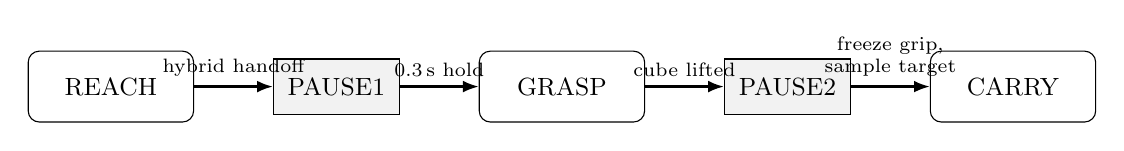
\begin{tikzpicture}[
    node distance=1.1cm and 1.0cm,
    every node/.style={font=\small},
    phase/.style={draw, rounded corners, minimum width=2.1cm, minimum height=0.9cm, align=center},
    pause/.style={draw, rectangle, minimum width=1.6cm, minimum height=0.7cm, align=center, fill=black!5},
    arr/.style={-{Latex[length=2mm]}, thick}
]
\node[phase] (reach) {REACH};
\node[pause, right=of reach] (p1) {PAUSE1};
\node[phase, right=of p1] (grasp) {GRASP};
\node[pause, right=of grasp] (p2) {PAUSE2};
\node[phase, right=of p2] (carry) {CARRY};

\draw[arr] (reach) -- (p1) node[midway, above, font=\scriptsize] {hybrid handoff};
\draw[arr] (p1) -- (grasp) node[midway, above, font=\scriptsize] {0.3\,s hold};
\draw[arr] (grasp) -- (p2) node[midway, above, font=\scriptsize] {cube lifted};
\draw[arr] (p2) -- (carry) node[midway, above, font=\scriptsize, align=center] {freeze grip,\\sample target};
\end{tikzpicture}
\end{center}

Every value below is a field of the \url{ChainCfg} dataclass in
\url{scripts/rsl_rl/lift_and_place_cfg.py}:

\begin{itemize}
    \item \textbf{Reach $\to$ Pause1 (hybrid handoff --- whichever fires first):}
    \begin{itemize}
        \item close and settled (\url{handoff_dist}, \url{handoff_speed}):
        distance to target $< 0.05$\,m \emph{and}
        end-effector speed $< 0.03$\,m/s; or
        \item plateaued (\url{handoff_plateau_steps}, \url{handoff_accept_dist}):
        no further progress for 30 steps ($\approx$1\,s)
        \emph{and} distance $< 0.07$\,m; or
        \item a hard timeout (\url{reach_timeout}) of 120 steps ($\approx$4\,s), so the chain always
        proceeds rather than stalling indefinitely on a poor approach.
    \end{itemize}
    \item \textbf{Pause1 $\to$ Grasp:} a fixed \url{pause_after_reach}$=0.3$\,s hold (reach policy keeps
    holding position) before handing control to grasp.
    \item \textbf{Grasp $\to$ Pause2:} triggers when the cube's height is within
    \url{grasp_lift_tol}$=2$\,cm of the \url{grasp_lift_z}$=0.155$\,m lift target. There is no timeout on this transition --- a
    grasp attempt that has not yet lifted the cube keeps trying until the episode
    itself ends.
    \item \textbf{Pause2 $\to$ Carry:} after a fixed \url{pause_after_grasp}$=0.1$\,s hold, the gripper command is
    frozen at grasp's last (closed) value, and a random carry target is sampled.
    \item \textbf{Carry:} the reach policy drives to a randomly sampled top-down
    pose in the air, sampled uniformly inside the box
    \url{air_x}$\,=[0.40, 0.60]$, \url{air_y}$\,=[-0.25, 0.25]$,
    \url{air_z}$\,=[0.25, 0.40]$\,m (pitch kept within reach's own trained orientation range,
    $[120^\circ, 180^\circ]$, to avoid out-of-distribution behavior). This box is
    sampled by the play script itself (\url{set_air_target} in
    \url{play_lift_and_place.py}); the chain environment's own
    \url{commands.object_pose.ranges} is a different, unrelated range left over
    from the single-policy \url{Gen3-LiftAndPlace-v0} task and is not what the
    carry target is actually drawn from, since the environment's built-in
    resampling for that command is disabled (\url{resampling_time_range} set to
    $10^9$\,s) precisely so the play script can own it.
\end{itemize}

\subsection{Timing unification and action clipping}

Because the chain runs two independently trained policies inside one simulated
environment, their simulation timing had to be made identical: both the grasp
environment and the chain environment use $dt = 1/60$\,s with a control decimation
of 2, matching the timing the reach policy itself was trained under. Each policy's
own trained action-clipping bound (read from its saved \url{agent.yaml}, e.g.\
grasp's $\pm1.0$; reach has none) is applied to that policy's raw output immediately after
inference via \url{.clamp()}, and the two clipped action tensors are merged by the current phase
using \url{torch.where} (\url{play_lift_and_place.py}) before being sent to the simulator.

\subsection{Visualization}

The chain overlays colored target markers so the active goal is visible during
playback (e.g.\ the current reach target and the carry target), and the fully
tuned version of the chain script and environment shortened the episode length from
10.0\,s to 5.0\,s and the post-grasp pause from 0.3\,s to 0.1\,s
(both changed together in the same tuning pass)
so that episodes
don't idle at the carry target for the remainder of their length, alongside a
marker-color and default-debug-sphere cleanup for cleaner recordings.

This tuning and the vision work described in Section~\ref{sec:vision} were originally developed
on separate branches that had diverged from each other; both have since been
reconciled into a single history on \url{main}, so the vision-enabled chain now uses the same
tuned timing and marker values described above.

% =====================================================================
\section{Results Summary}
\label{sec:results}
% =====================================================================

\subsection{Training curves}

Both the reach and grasp policies were trained multiple times as the reward
structure and randomization were iterated on; the runs referenced below are the
final, currently deployed checkpoints (Table~\ref{tab:reach_ppo}/\ref{tab:grasp_ppo}
give their exact training configuration).

\textbf{Reach.} Across training, the fine-grained position-tracking reward rises
from near zero ($\approx 0.0003$) to $\approx 0.33$--$0.36$; the fine-grained
orientation-tracking reward rises to $\approx 0.16$--$0.19$; the mean episode
reward rises from roughly $-0.2$ to $+4.0$--$4.5$. Essentially all episodes run to
the time-out termination (fraction $\approx 1.0$), i.e.\ reach has no meaningful
early-failure termination mode.

\textbf{Grasp.} Across the robustness-retrain runs, the \url{lifting_object}
reward (mean per-step ``cube is lifted'' signal, max 1.0 if lifted at every step)
rises from $\approx 0$ to $0.87$--$0.88$; the fine-grained \url{cube_to_target}
reward rises to $0.21$--$0.57$ depending on the run; the object-dropping
termination fraction (Isaac Lab's inherited \url{object_dropping} term,
triggered when the cube falls below $-0.05$\,m) stays low, $0.0016$--$0.0064$, i.e.\ dropping the cube after
picking it up is rare by the end of training; mean episode reward rises to
$3.97$--$6.37$.

\subsection{Qualitative results}

The full chain --- reach, grasp, and carry --- \textbf{works end-to-end}, and a
screen-recorded demo of a full pick-and-place rollout is committed to the
repository at \url{medias/kinova_video.mp4} and embedded in the project
README. ``Works end-to-end'' is, at this stage, a qualitative, video-verified
claim rather than a measured success percentage over $N$ episodes; Section~\ref{sec:vision}
does report a live running success fraction for the vision-driven chain, but it is a
console readout during play, not a value saved anywhere in the repository, so it is
likewise not a persisted statistic.

% =====================================================================
\section{Vision-Based Cube Pose Estimation}
\label{sec:vision}
% =====================================================================

\subsection{Motivation}

Every policy described so far conditions on the cube's pose as computed from
\textbf{privileged simulator state} (in earlier stages, via ground-truth object
pose and IK; described in the project's working notes as ``ground truth used to
set the reach/grasp targets''). The vision phase of the project replaces this
privileged signal with a pose estimate produced by a neural network observing a
single fixed RGB camera, so that the pipeline no longer depends on simulator-only
information.

\subsection{Camera setup}

A fixed \url{CameraCfg} was added to the chain environment
(\url{source/gen3/gen3/tasks/manager_based/gen3_lift_and_place/joint_pos_env_cfg.py},
in \url{Gen3LiftAndPlaceEnvCfg}, inherited by the chain subclasses): a pinhole camera at
world position $(1.319, 0, 1.153)$, oriented to look down at approximately
$(0.45, 0, 0.055)$ with roughly a $50^\circ$ downward tilt, focal length 24\,mm,
20.955\,mm horizontal aperture, clipping range $[0.1, 4.0]$\,m, capturing
$640\times480$ RGB frames. The placement was deliberately chosen to sit beyond the
cube's reachable $x$-range and centered in $y$, so that the descending gripper
does not fully occlude the cube from view during the grasp phase. A further
implementation detail worth noting: because the robot's base sits at the world
origin with identity rotation, the camera's world-frame pose \emph{is} already its
extrinsics in the robot-root frame that both policies are trained in, avoiding an
extra frame-conversion step downstream.

\subsection{Data collection}

The data-collection script,
\url{scripts/rsl_rl/vision/collect_vision_data.py}, runs the same frozen
reach~$\to$~pause1~$\to$~grasp~$\to$~pause2~$\to$~carry state machine used for
playback, across 32 parallel environments by default, and saves a frame and label
at (almost) every step instead of only rendering. The two near-static pause phases
are subsampled 1-in-\url{PAUSE_SAVE_STRIDE} (=5) to avoid wasting the dataset on near-duplicate frames, while
REACH/GRASP/CARRY frames are saved every step; a ``settled'' latch stops saving
further CARRY frames for an environment once its cube has arrived and stopped
moving, to the same end. Each collected frame is saved as an RGB PNG, and a
corresponding entry is appended to \url{labels.jsonl} recording the environment
id, simulation step, current phase, the cube's position and orientation
(quaternion) in the robot-root frame, and eight projected 2D cube-corner pixel
coordinates (a hand-written pinhole projection, kept for a possible future
keypoint/PnP-based approach but not used by the model actually trained). A single
\url{meta.json} records image resolution, the camera's intrinsic matrix, and its
extrinsics in the robot-root frame, written once from the live simulated camera at
collection time (not hand-entered).

The dataset actually present under \url{vision_dataset/} at the time of this
report (12{,}000 labeled frames, gitignored --- regenerable but not committed, so a
fresh collection run would produce a different random sample of similar size and
composition) was read directly to verify its phase distribution: \textbf{12{,}000 frames}
total, split 6494 \textsc{Carry}, 3320 \textsc{Reach},
2065 \textsc{Grasp}, 64 \textsc{Pause1}, 57 \textsc{Pause2} --- counted directly
from \url{labels.jsonl}, not recalled from notes.

\subsection{Dataset splitting}

\url{scripts/rsl_rl/vision/split_vision_dataset.py} performs a fixed-count random
split, not an exact phase-stratified one: records are shuffled with a fixed seed
(42) and then sliced into 1000 test / 1000 validation / 10{,}000 train frames ---
verified directly against the \url{train_labels.jsonl} / \url{val_labels.jsonl}
/ \url{test_labels.jsonl} files present in \url{vision_dataset/}. Shuffling before slicing (rather than splitting along rollout order, which would
front-load REACH frames) means each split ends up with a broadly representative mix
of phases in practice, and the script prints a per-split phase count as a sanity
check, but it does not explicitly enforce matching phase proportions across
splits.

\subsection{CubePoseNet: architecture}

The canonical \url{CubePoseNet} class is defined in
\url{scripts/rsl_rl/vision/train_cube_pose.py}: an ImageNet-pretrained \textbf{ResNet-18}
(He et al., 2016) backbone with its final
classification layer replaced by an identity mapping, feeding a small MLP head
($512 \to 256 \to 9$, ReLU) on top. The 9-dimensional output is split into a 3D
position and a \textbf{6D continuous rotation representation} (Zhou et al., 2019),
decoded into a full $3\times3$ rotation matrix via
Gram-Schmidt orthogonalization. This representation was chosen explicitly over
quaternions to avoid the antipodal sign ambiguity that quaternions introduce for
regression losses. Input frames are resized to $240\times320$ (the camera's native
capture resolution is $640\times480$; this resize happens at training/inference
time), ImageNet-normalized,
and (at training time only) augmented with color jitter (brightness, contrast,
saturation $\pm0.2$, hue $\pm0.02$). For live inference inside the chain, the
environment's vision observation module,
\url{source/gen3/gen3/tasks/manager_based/gen3_lift_and_place/mdp/vision_obs.py},
defines its own architecturally identical copy, \url{_CubePoseNet} --- its
docstring states explicitly that it ``must match \url{CubePoseNet} in
\url{scripts/rsl_rl/vision/train_cube_pose.py} exactly'' since a trained
checkpoint's \url{state_dict} is loaded into it directly. This duplication
(rather than importing the training script's class into the environment package)
keeps the environment config free of training-script dependencies, but it is a
place a future change to the network architecture must be applied twice.

The network regresses \textbf{full 3-DoF orientation}, not merely yaw, on the
grounds that once the cube is gripped it tilts freely --- the training script's
own documentation notes that 84\% of \textsc{Carry}-phase frames are not
yaw-only --- and that the cube's distinctly colored faces make full orientation
observable from a single image in the first place.

\subsection{Training setup}

\url{scripts/rsl_rl/vision/train_cube_pose.py} trains \url{CubePoseNet} with
AdamW (Loshchilov \& Hutter, 2019) (learning rate $3\times10^{-4}$, weight decay $1\times10^{-4}$), a cosine
annealing schedule over 30 epochs, batch size 64, and mixed-precision training.
The loss is
\[
\mathcal{L} = \text{MSE}(\hat{p}, p) + 0.1 \cdot \text{MSE}(\hat{R}, R),
\]
i.e.\ mean-squared error on position plus a matrix-MSE term on the rotation matrix
(weighted $0.1\times$) --- a simple Frobenius-style penalty at training time,
though rotation \emph{evaluation} is reported in degrees via a proper geodesic
error metric ($\arccos$ of the normalized trace of the relative rotation). Both the last and best (lowest validation position error) checkpoints
are saved each epoch; only the best checkpoint,
\url{pretrained_models/cube_pose/best.pt} (43.2\,MiB / 45.3\,MB on disk), is kept in the
repository.

\subsection{Results}

On the held-out, never-trained-on 1000-frame test split, \url{CubePoseNet}
achieves:
\[
\textbf{0.50\,cm position error, 1.2\textdegree{} rotation error}
\]
These headline numbers were independently reproduced while preparing this
revision by re-running
\url{scripts/rsl_rl/vision/eval_cube_pose.py} against the shipped
\url{pretrained_models/cube_pose/best.pt} checkpoint and the test split present
in \url{vision_dataset/}, not merely carried over from an earlier report.
That run's full per-phase breakdown (Table~\ref{tab:vision_phase}) is more precise
than a qualitative ``best/worst'' description: accuracy is not uniform across the
task, and while the coarsest characterization --- best on the table before the grasp, worst
right after the cube is lifted and partially occluded by the closed gripper --- still holds, \textsc{Pause1} (the settled moment just before grasp begins) is
in fact the single most accurate phase, and \textsc{Pause2} (holding the cube,
about to carry) the least accurate. Even the worst case (1.05\,cm) remains small
relative to the cube's own size ($\approx 7.2$\,cm).

\begin{table}[h]
\centering
\caption{\url{CubePoseNet} test-split accuracy per phase, measured directly by
re-running \url{eval_cube_pose.py} against \url{pretrained_models/cube_pose/best.pt}
(epoch 30, i.e.\ the fully trained checkpoint) on the 1000-frame test split.}
\label{tab:vision_phase}
\begin{tabular}{lcc}
\toprule
Phase & Position error (cm) & Rotation error ($^\circ$) \\
\midrule
All (overall) & 0.50 & 1.2 \\
Pause1 (settled, pre-grasp) & 0.27 & 0.6 \\
Reach & 0.42 & 0.9 \\
Carry & 0.50 & 1.1 \\
Grasp & 0.59 & 2.4 \\
Pause2 (holding, pre-carry) & 1.05 & 3.2 \\
\bottomrule
\end{tabular}
\end{table}

\subsection{Live integration into the chain}

This is not merely an offline-evaluated model: it is wired directly into a live
chain rollout. A new environment,
\url{Gen3-LiftAndPlace-Chain-Vision-v0}
(\url{gen3_lift_and_place/vision_env_cfg.py}, class
\url{Gen3LiftAndPlaceChainVisionEnvCfg}), subclasses the existing chain
environment and \textbf{overrides only the grasp policy's two cube-pose
observation terms} (\url{object_position} and \url{object_orientation})
with vision-based equivalents (\url{object_position_from_vision} /
\url{object_orientation_from_vision} in \url{mdp/vision_obs.py}) that call
\url{_CubePoseNet} on the live camera image --- reusing the exact same slot in the frozen grasp policy's observation
vector, so the policy itself is entirely unmodified; only the \emph{source} of
that observation changes. The model is loaded once and cached on the environment,
and its prediction is computed once per simulation step (cached, keyed by the
step counter) and shared by every
observation term and by the play script, rather than re-run redundantly.

\url{scripts/rsl_rl/play_lift_and_place.py} gained a \url{--vision} flag that switches to
this environment and replaces the ground-truth cube pose used for (a) the reach
target during the initial top-down approach, (b) the in-progress lift-height check
during grasp, and (c) the grasp$\to$pause2 transition condition, with the vision
model's live prediction (all three read through a single \url{cube_pose()}
helper in the play script that switches on \url{--vision}). The reach target is specifically \emph{re-sampled from
the latest prediction on every reach step}, not only once at episode reset, as an
explicit fix for one-step camera lag immediately following a reset. Ground truth is
retained only for a diagnostic prediction-error printout, not for any control
decision.

The vision-enabled play script does compute and print a running
(episodes-carried / episodes-completed) success fraction to the console as
episodes reset, but this is a live console readout, not a value that has been
captured and saved anywhere in the repository.

% =====================================================================
\section{Further Development}
\label{sec:further}
% =====================================================================

\subsection{Handling the Reach-Wavering Artifact}

The reach policy currently exhibits a small, persistent oscillation once it
settles at its target --- a learned wavering behavior present even under
deterministic evaluation, not exploration noise. Several reward-shaping
strategies (weak and strong joint-velocity penalties, both immediate and
curriculum-ramped, as well as a proximity-gated penalty) were tried and each ran
into the same tradeoff: any penalty strong enough to suppress the wavering also
suppressed the reach itself, since a velocity-based penalty cannot distinguish
approaching the target from oscillating at it. These specific attempts were not
preserved as separate commits (the current
\url{gen3_reach/joint_pos_env_cfg.py} reflects only the final, retained
smoothness curriculum described in Section~\ref{sec:reach}), so this account is
reconstructed from the project's own working notes rather than verifiable against
historical code; it is reported qualitatively for that reason, with no numerical
before/after claimed. The most promising direction not
yet attempted is at the \textbf{physics level} rather than the reward level: the
arm's wrist/elbow actuators are comparatively underdamped
(\url{source/gen3/gen3/assets/kinova_gen3_2f140.py}: damping 4.0/2.0 against
stiffness 60.0/25.0 for joints 1--4/5--7), and raising actuator damping should suppress the oscillation
directly without penalizing the reach itself. This would require retraining
reach under the new damping and re-validating the resulting control gains before
any hardware deployment.

\subsection{Sim-to-Real Deployment}

The project has been developed and validated entirely in simulation. Moving the
pick-and-place chain onto the physical Kinova Gen3 would need to address, at
minimum: matching the real arm's controller gains to the simulated
stiffness/damping values so trained behavior transfers (particularly if the
damping change above is made); calibrating the real camera's intrinsics and
extrinsics for \url{CubePoseNet}, which was trained only on rendered
simulation images and would need to be validated against, or fine-tuned on, real
camera images; and re-checking the Robotiq 2F-140's real actuation timing and
grip-force behavior, since its simulated model is only an approximation of the
physical gripper's dynamics. None of this has been attempted yet.

% =====================================================================
\section{Conclusion}
\label{sec:conclusion}
% =====================================================================

The project has produced a working, end-to-end simulated pick-and-place pipeline
on a Kinova Gen3 + Robotiq 2F-140 platform, composed from two independently
trained PPO policies (Sections~\ref{sec:reach}--\ref{sec:grasp}, trained with the
RSL-RL implementation of PPO within NVIDIA Isaac Lab --- Section~\ref{sec:background}
details this software boundary), and has extended that pipeline with a vision-based cube-pose
estimator that is already measured (0.50\,cm / 1.2\textdegree{} test-set error, independently
reproduced for this revision --- Section~\ref{sec:vision}) and
already wired into a live \url{--vision} chain mode. The items in Section~\ref{sec:further}
are the natural next steps for the project.

\end{document}
